\documentclass[parskip=half]{scrartcl}
        \usepackage{tikz}
        \usepackage{pxfonts}
        \usepackage[a4paper,left=1cm,right=1cm,top=2cm,bottom=3cm]{geometry}
        \title{Conformance Testing Report}
        \author{\relax}\date{\today}
        \begin{document} \maketitle
        \section{Benchmark information}
        \begin{tabular}{l|l} \
        \textbf{Benchmark name:} & ImageNet-val \\ \hline
        \textbf{Model:} & resnet50 (ResNet50_Weights.IMAGENET1K_V1, pretrained, no training) \\ \hline
        \textbf{Augmentations:} & [{}, {'degree': np.float64(-179.0)}, {'degree': np.float64(-178.0)}, {'degree': np.float64(-177.0)}, {'degree': np.float64(-176.0)}, {'degree': np.float64(-175.0)}, {'degree': np.float64(-174.0)}, {'degree': np.float64(-173.0)}, {'degree': np.float64(-172.0)}, {'degree': np.float64(-171.0)}, {'degree': np.float64(-170.0)}, {'degree': np.float64(-169.0)}, {'degree': np.float64(-168.0)}, {'degree': np.float64(-167.0)}, {'degree': np.float64(-166.0)}, {'degree': np.float64(-165.0)}, {'degree': np.float64(-164.0)}, {'degree': np.float64(-163.0)}, {'degree': np.float64(-162.0)}, {'degree': np.float64(-161.0)}, {'degree': np.float64(-160.0)}, {'degree': np.float64(-159.0)}, {'degree': np.float64(-158.0)}, {'degree': np.float64(-157.0)}, {'degree': np.float64(-156.0)}, {'degree': np.float64(-155.0)}, {'degree': np.float64(-154.0)}, {'degree': np.float64(-153.0)}, {'degree': np.float64(-152.0)}, {'degree': np.float64(-151.0)}, {'degree': np.float64(-150.0)}, {'degree': np.float64(-149.0)}, {'degree': np.float64(-148.0)}, {'degree': np.float64(-147.0)}, {'degree': np.float64(-146.0)}, {'degree': np.float64(-145.0)}, {'degree': np.float64(-144.0)}, {'degree': np.float64(-143.0)}, {'degree': np.float64(-142.0)}, {'degree': np.float64(-141.0)}, {'degree': np.float64(-140.0)}, {'degree': np.float64(-139.0)}, {'degree': np.float64(-138.0)}, {'degree': np.float64(-137.0)}, {'degree': np.float64(-136.0)}, {'degree': np.float64(-135.0)}, {'degree': np.float64(-134.0)}, {'degree': np.float64(-133.0)}, {'degree': np.float64(-132.0)}, {'degree': np.float64(-131.0)}, {'degree': np.float64(-130.0)}, {'degree': np.float64(-129.0)}, {'degree': np.float64(-128.0)}, {'degree': np.float64(-127.0)}, {'degree': np.float64(-126.0)}, {'degree': np.float64(-125.0)}, {'degree': np.float64(-124.0)}, {'degree': np.float64(-123.0)}, {'degree': np.float64(-122.0)}, {'degree': np.float64(-121.0)}, {'degree': np.float64(-120.0)}, {'degree': np.float64(-119.0)}, {'degree': np.float64(-118.0)}, {'degree': np.float64(-117.0)}, {'degree': np.float64(-116.0)}, {'degree': np.float64(-115.0)}, {'degree': np.float64(-114.0)}, {'degree': np.float64(-113.0)}, {'degree': np.float64(-112.0)}, {'degree': np.float64(-111.0)}, {'degree': np.float64(-110.0)}, {'degree': np.float64(-109.0)}, {'degree': np.float64(-108.0)}, {'degree': np.float64(-107.0)}, {'degree': np.float64(-106.0)}, {'degree': np.float64(-105.0)}, {'degree': np.float64(-104.0)}, {'degree': np.float64(-103.0)}, {'degree': np.float64(-102.0)}, {'degree': np.float64(-101.0)}, {'degree': np.float64(-100.0)}, {'degree': np.float64(-99.0)}, {'degree': np.float64(-98.0)}, {'degree': np.float64(-97.0)}, {'degree': np.float64(-96.0)}, {'degree': np.float64(-95.0)}, {'degree': np.float64(-94.0)}, {'degree': np.float64(-93.0)}, {'degree': np.float64(-92.0)}, {'degree': np.float64(-91.0)}, {'degree': np.float64(-90.0)}, {'degree': np.float64(-89.0)}, {'degree': np.float64(-88.0)}, {'degree': np.float64(-87.0)}, {'degree': np.float64(-86.0)}, {'degree': np.float64(-85.0)}, {'degree': np.float64(-84.0)}, {'degree': np.float64(-83.0)}, {'degree': np.float64(-82.0)}, {'degree': np.float64(-81.0)}, {'degree': np.float64(-80.0)}, {'degree': np.float64(-79.0)}, {'degree': np.float64(-78.0)}, {'degree': np.float64(-77.0)}, {'degree': np.float64(-76.0)}, {'degree': np.float64(-75.0)}, {'degree': np.float64(-74.0)}, {'degree': np.float64(-73.0)}, {'degree': np.float64(-72.0)}, {'degree': np.float64(-71.0)}, {'degree': np.float64(-70.0)}, {'degree': np.float64(-69.0)}, {'degree': np.float64(-68.0)}, {'degree': np.float64(-67.0)}, {'degree': np.float64(-66.0)}, {'degree': np.float64(-65.0)}, {'degree': np.float64(-64.0)}, {'degree': np.float64(-63.0)}, {'degree': np.float64(-62.0)}, {'degree': np.float64(-61.0)}, {'degree': np.float64(-60.0)}, {'degree': np.float64(-59.0)}, {'degree': np.float64(-58.0)}, {'degree': np.float64(-57.0)}, {'degree': np.float64(-56.0)}, {'degree': np.float64(-55.0)}, {'degree': np.float64(-54.0)}, {'degree': np.float64(-53.0)}, {'degree': np.float64(-52.0)}, {'degree': np.float64(-51.0)}, {'degree': np.float64(-50.0)}, {'degree': np.float64(-49.0)}, {'degree': np.float64(-48.0)}, {'degree': np.float64(-47.0)}, {'degree': np.float64(-46.0)}, {'degree': np.float64(-45.0)}, {'degree': np.float64(-44.0)}, {'degree': np.float64(-43.0)}, {'degree': np.float64(-42.0)}, {'degree': np.float64(-41.0)}, {'degree': np.float64(-40.0)}, {'degree': np.float64(-39.0)}, {'degree': np.float64(-38.0)}, {'degree': np.float64(-37.0)}, {'degree': np.float64(-36.0)}, {'degree': np.float64(-35.0)}, {'degree': np.float64(-34.0)}, {'degree': np.float64(-33.0)}, {'degree': np.float64(-32.0)}, {'degree': np.float64(-31.0)}, {'degree': np.float64(-30.0)}, {'degree': np.float64(-29.0)}, {'degree': np.float64(-28.0)}, {'degree': np.float64(-27.0)}, {'degree': np.float64(-26.0)}, {'degree': np.float64(-25.0)}, {'degree': np.float64(-24.0)}, {'degree': np.float64(-23.0)}, {'degree': np.float64(-22.0)}, {'degree': np.float64(-21.0)}, {'degree': np.float64(-20.0)}, {'degree': np.float64(-19.0)}, {'degree': np.float64(-18.0)}, {'degree': np.float64(-17.0)}, {'degree': np.float64(-16.0)}, {'degree': np.float64(-15.0)}, {'degree': np.float64(-14.0)}, {'degree': np.float64(-13.0)}, {'degree': np.float64(-12.0)}, {'degree': np.float64(-11.0)}, {'degree': np.float64(-10.0)}, {'degree': np.float64(-9.0)}, {'degree': np.float64(-8.0)}, {'degree': np.float64(-7.0)}, {'degree': np.float64(-6.0)}, {'degree': np.float64(-5.0)}, {'degree': np.float64(-4.0)}, {'degree': np.float64(-3.0)}, {'degree': np.float64(-2.0)}, {'degree': np.float64(-1.0)}, {'degree': np.float64(1.0)}, {'degree': np.float64(2.0)}, {'degree': np.float64(3.0)}, {'degree': np.float64(4.0)}, {'degree': np.float64(5.0)}, {'degree': np.float64(6.0)}, {'degree': np.float64(7.0)}, {'degree': np.float64(8.0)}, {'degree': np.float64(9.0)}, {'degree': np.float64(10.0)}, {'degree': np.float64(11.0)}, {'degree': np.float64(12.0)}, {'degree': np.float64(13.0)}, {'degree': np.float64(14.0)}, {'degree': np.float64(15.0)}, {'degree': np.float64(16.0)}, {'degree': np.float64(17.0)}, {'degree': np.float64(18.0)}, {'degree': np.float64(19.0)}, {'degree': np.float64(20.0)}, {'degree': np.float64(21.0)}, {'degree': np.float64(22.0)}, {'degree': np.float64(23.0)}, {'degree': np.float64(24.0)}, {'degree': np.float64(25.0)}, {'degree': np.float64(26.0)}, {'degree': np.float64(27.0)}, {'degree': np.float64(28.0)}, {'degree': np.float64(29.0)}, {'degree': np.float64(30.0)}, {'degree': np.float64(31.0)}, {'degree': np.float64(32.0)}, {'degree': np.float64(33.0)}, {'degree': np.float64(34.0)}, {'degree': np.float64(35.0)}, {'degree': np.float64(36.0)}, {'degree': np.float64(37.0)}, {'degree': np.float64(38.0)}, {'degree': np.float64(39.0)}, {'degree': np.float64(40.0)}, {'degree': np.float64(41.0)}, {'degree': np.float64(42.0)}, {'degree': np.float64(43.0)}, {'degree': np.float64(44.0)}, {'degree': np.float64(45.0)}, {'degree': np.float64(46.0)}, {'degree': np.float64(47.0)}, {'degree': np.float64(48.0)}, {'degree': np.float64(49.0)}, {'degree': np.float64(50.0)}, {'degree': np.float64(51.0)}, {'degree': np.float64(52.0)}, {'degree': np.float64(53.0)}, {'degree': np.float64(54.0)}, {'degree': np.float64(55.0)}, {'degree': np.float64(56.0)}, {'degree': np.float64(57.0)}, {'degree': np.float64(58.0)}, {'degree': np.float64(59.0)}, {'degree': np.float64(60.0)}, {'degree': np.float64(61.0)}, {'degree': np.float64(62.0)}, {'degree': np.float64(63.0)}, {'degree': np.float64(64.0)}, {'degree': np.float64(65.0)}, {'degree': np.float64(66.0)}, {'degree': np.float64(67.0)}, {'degree': np.float64(68.0)}, {'degree': np.float64(69.0)}, {'degree': np.float64(70.0)}, {'degree': np.float64(71.0)}, {'degree': np.float64(72.0)}, {'degree': np.float64(73.0)}, {'degree': np.float64(74.0)}, {'degree': np.float64(75.0)}, {'degree': np.float64(76.0)}, {'degree': np.float64(77.0)}, {'degree': np.float64(78.0)}, {'degree': np.float64(79.0)}, {'degree': np.float64(80.0)}, {'degree': np.float64(81.0)}, {'degree': np.float64(82.0)}, {'degree': np.float64(83.0)}, {'degree': np.float64(84.0)}, {'degree': np.float64(85.0)}, {'degree': np.float64(86.0)}, {'degree': np.float64(87.0)}, {'degree': np.float64(88.0)}, {'degree': np.float64(89.0)}, {'degree': np.float64(90.0)}, {'degree': np.float64(91.0)}, {'degree': np.float64(92.0)}, {'degree': np.float64(93.0)}, {'degree': np.float64(94.0)}, {'degree': np.float64(95.0)}, {'degree': np.float64(96.0)}, {'degree': np.float64(97.0)}, {'degree': np.float64(98.0)}, {'degree': np.float64(99.0)}, {'degree': np.float64(100.0)}, {'degree': np.float64(101.0)}, {'degree': np.float64(102.0)}, {'degree': np.float64(103.0)}, {'degree': np.float64(104.0)}, {'degree': np.float64(105.0)}, {'degree': np.float64(106.0)}, {'degree': np.float64(107.0)}, {'degree': np.float64(108.0)}, {'degree': np.float64(109.0)}, {'degree': np.float64(110.0)}, {'degree': np.float64(111.0)}, {'degree': np.float64(112.0)}, {'degree': np.float64(113.0)}, {'degree': np.float64(114.0)}, {'degree': np.float64(115.0)}, {'degree': np.float64(116.0)}, {'degree': np.float64(117.0)}, {'degree': np.float64(118.0)}, {'degree': np.float64(119.0)}, {'degree': np.float64(120.0)}, {'degree': np.float64(121.0)}, {'degree': np.float64(122.0)}, {'degree': np.float64(123.0)}, {'degree': np.float64(124.0)}, {'degree': np.float64(125.0)}, {'degree': np.float64(126.0)}, {'degree': np.float64(127.0)}, {'degree': np.float64(128.0)}, {'degree': np.float64(129.0)}, {'degree': np.float64(130.0)}, {'degree': np.float64(131.0)}, {'degree': np.float64(132.0)}, {'degree': np.float64(133.0)}, {'degree': np.float64(134.0)}, {'degree': np.float64(135.0)}, {'degree': np.float64(136.0)}, {'degree': np.float64(137.0)}, {'degree': np.float64(138.0)}, {'degree': np.float64(139.0)}, {'degree': np.float64(140.0)}, {'degree': np.float64(141.0)}, {'degree': np.float64(142.0)}, {'degree': np.float64(143.0)}, {'degree': np.float64(144.0)}, {'degree': np.float64(145.0)}, {'degree': np.float64(146.0)}, {'degree': np.float64(147.0)}, {'degree': np.float64(148.0)}, {'degree': np.float64(149.0)}, {'degree': np.float64(150.0)}, {'degree': np.float64(151.0)}, {'degree': np.float64(152.0)}, {'degree': np.float64(153.0)}, {'degree': np.float64(154.0)}, {'degree': np.float64(155.0)}, {'degree': np.float64(156.0)}, {'degree': np.float64(157.0)}, {'degree': np.float64(158.0)}, {'degree': np.float64(159.0)}, {'degree': np.float64(160.0)}, {'degree': np.float64(161.0)}, {'degree': np.float64(162.0)}, {'degree': np.float64(163.0)}, {'degree': np.float64(164.0)}, {'degree': np.float64(165.0)}, {'degree': np.float64(166.0)}, {'degree': np.float64(167.0)}, {'degree': np.float64(168.0)}, {'degree': np.float64(169.0)}, {'degree': np.float64(170.0)}, {'degree': np.float64(171.0)}, {'degree': np.float64(172.0)}, {'degree': np.float64(173.0)}, {'degree': np.float64(174.0)}, {'degree': np.float64(175.0)}, {'degree': np.float64(176.0)}, {'degree': np.float64(177.0)}, {'degree': np.float64(178.0)}, {'degree': np.float64(179.0)}] \\ \hline
        \textbf{Top-1 accuracy (test split):} & ORIGINAL: 76.22\% / ROTATE_PROBE_-179.0: 49.75\% / ROTATE_PROBE_-178.0: 48.07\% / ROTATE_PROBE_-177.0: 45.84\% / ROTATE_PROBE_-176.0: 44.62\% / ROTATE_PROBE_-175.0: 42.84\% / ROTATE_PROBE_-174.0: 40.02\% / ROTATE_PROBE_-173.0: 37.87\% / ROTATE_PROBE_-172.0: 36.03\% / ROTATE_PROBE_-171.0: 34.2\% / ROTATE_PROBE_-170.0: 32.14\% / ROTATE_PROBE_-169.0: 30.75\% / ROTATE_PROBE_-168.0: 29.27\% / ROTATE_PROBE_-167.0: 28.19\% / ROTATE_PROBE_-166.0: 27.53\% / ROTATE_PROBE_-165.0: 26.1\% / ROTATE_PROBE_-164.0: 24.87\% / ROTATE_PROBE_-163.0: 23.76\% / ROTATE_PROBE_-162.0: 23.51\% / ROTATE_PROBE_-161.0: 22.39\% / ROTATE_PROBE_-160.0: 22.6\% / ROTATE_PROBE_-159.0: 22.14\% / ROTATE_PROBE_-158.0: 22.0\% / ROTATE_PROBE_-157.0: 22.46\% / ROTATE_PROBE_-156.0: 22.76\% / ROTATE_PROBE_-155.0: 23.54\% / ROTATE_PROBE_-154.0: 23.97\% / ROTATE_PROBE_-153.0: 24.05\% / ROTATE_PROBE_-152.0: 24.44\% / ROTATE_PROBE_-151.0: 24.27\% / ROTATE_PROBE_-150.0: 24.14\% / ROTATE_PROBE_-149.0: 23.92\% / ROTATE_PROBE_-148.0: 23.86\% / ROTATE_PROBE_-147.0: 24.07\% / ROTATE_PROBE_-146.0: 23.97\% / ROTATE_PROBE_-145.0: 24.7\% / ROTATE_PROBE_-144.0: 25.07\% / ROTATE_PROBE_-143.0: 24.72\% / ROTATE_PROBE_-142.0: 25.3\% / ROTATE_PROBE_-141.0: 25.87\% / ROTATE_PROBE_-140.0: 26.14\% / ROTATE_PROBE_-139.0: 26.46\% / ROTATE_PROBE_-138.0: 27.52\% / ROTATE_PROBE_-137.0: 28.47\% / ROTATE_PROBE_-136.0: 30.06\% / ROTATE_PROBE_-135.0: 31.72\% / ROTATE_PROBE_-134.0: 29.76\% / ROTATE_PROBE_-133.0: 28.31\% / ROTATE_PROBE_-132.0: 27.73\% / ROTATE_PROBE_-131.0: 26.79\% / ROTATE_PROBE_-130.0: 26.18\% / ROTATE_PROBE_-129.0: 25.94\% / ROTATE_PROBE_-128.0: 25.86\% / ROTATE_PROBE_-127.0: 24.99\% / ROTATE_PROBE_-126.0: 25.01\% / ROTATE_PROBE_-125.0: 24.39\% / ROTATE_PROBE_-124.0: 24.04\% / ROTATE_PROBE_-123.0: 23.82\% / ROTATE_PROBE_-122.0: 24.09\% / ROTATE_PROBE_-121.0: 24.06\% / ROTATE_PROBE_-120.0: 24.7\% / ROTATE_PROBE_-119.0: 24.59\% / ROTATE_PROBE_-118.0: 25.05\% / ROTATE_PROBE_-117.0: 24.52\% / ROTATE_PROBE_-116.0: 24.38\% / ROTATE_PROBE_-115.0: 23.99\% / ROTATE_PROBE_-114.0: 23.34\% / ROTATE_PROBE_-113.0: 22.81\% / ROTATE_PROBE_-112.0: 22.51\% / ROTATE_PROBE_-111.0: 22.36\% / ROTATE_PROBE_-110.0: 22.4\% / ROTATE_PROBE_-109.0: 22.61\% / ROTATE_PROBE_-108.0: 23.27\% / ROTATE_PROBE_-107.0: 23.86\% / ROTATE_PROBE_-106.0: 25.0\% / ROTATE_PROBE_-105.0: 25.71\% / ROTATE_PROBE_-104.0: 26.74\% / ROTATE_PROBE_-103.0: 27.32\% / ROTATE_PROBE_-102.0: 28.36\% / ROTATE_PROBE_-101.0: 29.57\% / ROTATE_PROBE_-100.0: 31.15\% / ROTATE_PROBE_-99.0: 32.86\% / ROTATE_PROBE_-98.0: 34.53\% / ROTATE_PROBE_-97.0: 36.06\% / ROTATE_PROBE_-96.0: 38.54\% / ROTATE_PROBE_-95.0: 41.26\% / ROTATE_PROBE_-94.0: 43.14\% / ROTATE_PROBE_-93.0: 44.78\% / ROTATE_PROBE_-92.0: 46.71\% / ROTATE_PROBE_-91.0: 48.61\% / ROTATE_PROBE_-90.0: 50.52\% / ROTATE_PROBE_-89.0: 49.5\% / ROTATE_PROBE_-88.0: 47.42\% / ROTATE_PROBE_-87.0: 45.58\% / ROTATE_PROBE_-86.0: 44.47\% / ROTATE_PROBE_-85.0: 42.71\% / ROTATE_PROBE_-84.0: 40.56\% / ROTATE_PROBE_-83.0: 38.94\% / ROTATE_PROBE_-82.0: 36.99\% / ROTATE_PROBE_-81.0: 35.94\% / ROTATE_PROBE_-80.0: 34.58\% / ROTATE_PROBE_-79.0: 33.37\% / ROTATE_PROBE_-78.0: 32.85\% / ROTATE_PROBE_-77.0: 31.88\% / ROTATE_PROBE_-76.0: 31.74\% / ROTATE_PROBE_-75.0: 30.94\% / ROTATE_PROBE_-74.0: 30.1\% / ROTATE_PROBE_-73.0: 29.34\% / ROTATE_PROBE_-72.0: 29.13\% / ROTATE_PROBE_-71.0: 28.34\% / ROTATE_PROBE_-70.0: 28.64\% / ROTATE_PROBE_-69.0: 29.21\% / ROTATE_PROBE_-68.0: 29.42\% / ROTATE_PROBE_-67.0: 30.3\% / ROTATE_PROBE_-66.0: 30.82\% / ROTATE_PROBE_-65.0: 32.32\% / ROTATE_PROBE_-64.0: 33.22\% / ROTATE_PROBE_-63.0: 33.73\% / ROTATE_PROBE_-62.0: 34.44\% / ROTATE_PROBE_-61.0: 34.26\% / ROTATE_PROBE_-60.0: 34.5\% / ROTATE_PROBE_-59.0: 34.84\% / ROTATE_PROBE_-58.0: 34.56\% / ROTATE_PROBE_-57.0: 35.33\% / ROTATE_PROBE_-56.0: 35.53\% / ROTATE_PROBE_-55.0: 36.34\% / ROTATE_PROBE_-54.0: 37.57\% / ROTATE_PROBE_-53.0: 37.75\% / ROTATE_PROBE_-52.0: 39.0\% / ROTATE_PROBE_-51.0: 40.17\% / ROTATE_PROBE_-50.0: 40.98\% / ROTATE_PROBE_-49.0: 41.81\% / ROTATE_PROBE_-48.0: 43.61\% / ROTATE_PROBE_-47.0: 45.47\% / ROTATE_PROBE_-46.0: 46.94\% / ROTATE_PROBE_-45.0: 48.67\% / ROTATE_PROBE_-44.0: 47.32\% / ROTATE_PROBE_-43.0: 45.98\% / ROTATE_PROBE_-42.0: 45.78\% / ROTATE_PROBE_-41.0: 45.14\% / ROTATE_PROBE_-40.0: 45.24\% / ROTATE_PROBE_-39.0: 45.0\% / ROTATE_PROBE_-38.0: 45.06\% / ROTATE_PROBE_-37.0: 44.54\% / ROTATE_PROBE_-36.0: 44.66\% / ROTATE_PROBE_-35.0: 44.58\% / ROTATE_PROBE_-34.0: 44.77\% / ROTATE_PROBE_-33.0: 44.59\% / ROTATE_PROBE_-32.0: 45.25\% / ROTATE_PROBE_-31.0: 46.26\% / ROTATE_PROBE_-30.0: 47.07\% / ROTATE_PROBE_-29.0: 47.66\% / ROTATE_PROBE_-28.0: 47.9\% / ROTATE_PROBE_-27.0: 48.38\% / ROTATE_PROBE_-26.0: 48.58\% / ROTATE_PROBE_-25.0: 48.45\% / ROTATE_PROBE_-24.0: 47.7\% / ROTATE_PROBE_-23.0: 47.3\% / ROTATE_PROBE_-22.0: 47.14\% / ROTATE_PROBE_-21.0: 47.16\% / ROTATE_PROBE_-20.0: 47.26\% / ROTATE_PROBE_-19.0: 47.31\% / ROTATE_PROBE_-18.0: 48.18\% / ROTATE_PROBE_-17.0: 49.25\% / ROTATE_PROBE_-16.0: 50.62\% / ROTATE_PROBE_-15.0: 52.34\% / ROTATE_PROBE_-14.0: 53.75\% / ROTATE_PROBE_-13.0: 54.68\% / ROTATE_PROBE_-12.0: 56.26\% / ROTATE_PROBE_-11.0: 57.79\% / ROTATE_PROBE_-10.0: 59.4\% / ROTATE_PROBE_-9.0: 61.36\% / ROTATE_PROBE_-8.0: 62.96\% / ROTATE_PROBE_-7.0: 64.58\% / ROTATE_PROBE_-6.0: 66.81\% / ROTATE_PROBE_-5.0: 69.1\% / ROTATE_PROBE_-4.0: 70.33\% / ROTATE_PROBE_-3.0: 71.48\% / ROTATE_PROBE_-2.0: 73.3\% / ROTATE_PROBE_-1.0: 74.83\% / ROTATE_PROBE_1.0: 74.6\% / ROTATE_PROBE_2.0: 73.1\% / ROTATE_PROBE_3.0: 71.58\% / ROTATE_PROBE_4.0: 70.7\% / ROTATE_PROBE_5.0: 68.95\% / ROTATE_PROBE_6.0: 67.36\% / ROTATE_PROBE_7.0: 65.57\% / ROTATE_PROBE_8.0: 64.23\% / ROTATE_PROBE_9.0: 62.24\% / ROTATE_PROBE_10.0: 59.88\% / ROTATE_PROBE_11.0: 58.47\% / ROTATE_PROBE_12.0: 57.17\% / ROTATE_PROBE_13.0: 55.79\% / ROTATE_PROBE_14.0: 54.64\% / ROTATE_PROBE_15.0: 53.15\% / ROTATE_PROBE_16.0: 51.84\% / ROTATE_PROBE_17.0: 50.2\% / ROTATE_PROBE_18.0: 49.35\% / ROTATE_PROBE_19.0: 48.21\% / ROTATE_PROBE_20.0: 47.74\% / ROTATE_PROBE_21.0: 47.58\% / ROTATE_PROBE_22.0: 47.25\% / ROTATE_PROBE_23.0: 47.37\% / ROTATE_PROBE_24.0: 47.32\% / ROTATE_PROBE_25.0: 48.29\% / ROTATE_PROBE_26.0: 48.45\% / ROTATE_PROBE_27.0: 48.22\% / ROTATE_PROBE_28.0: 48.17\% / ROTATE_PROBE_29.0: 47.58\% / ROTATE_PROBE_30.0: 47.05\% / ROTATE_PROBE_31.0: 45.72\% / ROTATE_PROBE_32.0: 45.19\% / ROTATE_PROBE_33.0: 44.64\% / ROTATE_PROBE_34.0: 44.7\% / ROTATE_PROBE_35.0: 44.51\% / ROTATE_PROBE_36.0: 44.6\% / ROTATE_PROBE_37.0: 44.27\% / ROTATE_PROBE_38.0: 44.48\% / ROTATE_PROBE_39.0: 44.78\% / ROTATE_PROBE_40.0: 44.3\% / ROTATE_PROBE_41.0: 44.86\% / ROTATE_PROBE_42.0: 45.65\% / ROTATE_PROBE_43.0: 46.48\% / ROTATE_PROBE_44.0: 47.36\% / ROTATE_PROBE_45.0: 48.3\% / ROTATE_PROBE_46.0: 46.24\% / ROTATE_PROBE_47.0: 43.83\% / ROTATE_PROBE_48.0: 42.51\% / ROTATE_PROBE_49.0: 41.27\% / ROTATE_PROBE_50.0: 40.32\% / ROTATE_PROBE_51.0: 39.51\% / ROTATE_PROBE_52.0: 38.94\% / ROTATE_PROBE_53.0: 37.22\% / ROTATE_PROBE_54.0: 36.98\% / ROTATE_PROBE_55.0: 35.63\% / ROTATE_PROBE_56.0: 34.85\% / ROTATE_PROBE_57.0: 34.39\% / ROTATE_PROBE_58.0: 34.01\% / ROTATE_PROBE_59.0: 33.99\% / ROTATE_PROBE_60.0: 34.45\% / ROTATE_PROBE_61.0: 33.74\% / ROTATE_PROBE_62.0: 33.62\% / ROTATE_PROBE_63.0: 32.77\% / ROTATE_PROBE_64.0: 32.46\% / ROTATE_PROBE_65.0: 32.01\% / ROTATE_PROBE_66.0: 31.02\% / ROTATE_PROBE_67.0: 29.84\% / ROTATE_PROBE_68.0: 29.18\% / ROTATE_PROBE_69.0: 28.59\% / ROTATE_PROBE_70.0: 28.09\% / ROTATE_PROBE_71.0: 27.89\% / ROTATE_PROBE_72.0: 28.1\% / ROTATE_PROBE_73.0: 28.39\% / ROTATE_PROBE_74.0: 28.98\% / ROTATE_PROBE_75.0: 29.39\% / ROTATE_PROBE_76.0: 29.96\% / ROTATE_PROBE_77.0: 30.68\% / ROTATE_PROBE_78.0: 31.46\% / ROTATE_PROBE_79.0: 32.18\% / ROTATE_PROBE_80.0: 33.37\% / ROTATE_PROBE_81.0: 34.89\% / ROTATE_PROBE_82.0: 35.98\% / ROTATE_PROBE_83.0: 37.55\% / ROTATE_PROBE_84.0: 40.02\% / ROTATE_PROBE_85.0: 42.13\% / ROTATE_PROBE_86.0: 43.86\% / ROTATE_PROBE_87.0: 45.07\% / ROTATE_PROBE_88.0: 47.03\% / ROTATE_PROBE_89.0: 48.56\% / ROTATE_PROBE_90.0: 50.1\% / ROTATE_PROBE_91.0: 48.47\% / ROTATE_PROBE_92.0: 46.68\% / ROTATE_PROBE_93.0: 44.66\% / ROTATE_PROBE_94.0: 43.5\% / ROTATE_PROBE_95.0: 40.8\% / ROTATE_PROBE_96.0: 38.7\% / ROTATE_PROBE_97.0: 36.85\% / ROTATE_PROBE_98.0: 34.57\% / ROTATE_PROBE_99.0: 32.92\% / ROTATE_PROBE_100.0: 31.42\% / ROTATE_PROBE_101.0: 30.06\% / ROTATE_PROBE_102.0: 28.9\% / ROTATE_PROBE_103.0: 28.01\% / ROTATE_PROBE_104.0: 27.39\% / ROTATE_PROBE_105.0: 26.31\% / ROTATE_PROBE_106.0: 25.45\% / ROTATE_PROBE_107.0: 24.43\% / ROTATE_PROBE_108.0: 23.82\% / ROTATE_PROBE_109.0: 23.1\% / ROTATE_PROBE_110.0: 22.86\% / ROTATE_PROBE_111.0: 22.86\% / ROTATE_PROBE_112.0: 22.73\% / ROTATE_PROBE_113.0: 23.09\% / ROTATE_PROBE_114.0: 23.51\% / ROTATE_PROBE_115.0: 23.86\% / ROTATE_PROBE_116.0: 23.87\% / ROTATE_PROBE_117.0: 24.06\% / ROTATE_PROBE_118.0: 24.79\% / ROTATE_PROBE_119.0: 24.46\% / ROTATE_PROBE_120.0: 24.26\% / ROTATE_PROBE_121.0: 24.08\% / ROTATE_PROBE_122.0: 23.58\% / ROTATE_PROBE_123.0: 24.17\% / ROTATE_PROBE_124.0: 23.76\% / ROTATE_PROBE_125.0: 24.6\% / ROTATE_PROBE_126.0: 24.88\% / ROTATE_PROBE_127.0: 25.16\% / ROTATE_PROBE_128.0: 25.74\% / ROTATE_PROBE_129.0: 25.63\% / ROTATE_PROBE_130.0: 25.96\% / ROTATE_PROBE_131.0: 26.61\% / ROTATE_PROBE_132.0: 27.3\% / ROTATE_PROBE_133.0: 28.8\% / ROTATE_PROBE_134.0: 29.93\% / ROTATE_PROBE_135.0: 31.21\% / ROTATE_PROBE_136.0: 29.5\% / ROTATE_PROBE_137.0: 28.15\% / ROTATE_PROBE_138.0: 27.16\% / ROTATE_PROBE_139.0: 26.54\% / ROTATE_PROBE_140.0: 26.04\% / ROTATE_PROBE_141.0: 25.9\% / ROTATE_PROBE_142.0: 25.61\% / ROTATE_PROBE_143.0: 25.39\% / ROTATE_PROBE_144.0: 25.21\% / ROTATE_PROBE_145.0: 24.39\% / ROTATE_PROBE_146.0: 23.81\% / ROTATE_PROBE_147.0: 23.69\% / ROTATE_PROBE_148.0: 23.59\% / ROTATE_PROBE_149.0: 24.3\% / ROTATE_PROBE_150.0: 24.9\% / ROTATE_PROBE_151.0: 24.37\% / ROTATE_PROBE_152.0: 24.78\% / ROTATE_PROBE_153.0: 24.26\% / ROTATE_PROBE_154.0: 24.22\% / ROTATE_PROBE_155.0: 24.41\% / ROTATE_PROBE_156.0: 23.64\% / ROTATE_PROBE_157.0: 23.12\% / ROTATE_PROBE_158.0: 22.55\% / ROTATE_PROBE_159.0: 22.67\% / ROTATE_PROBE_160.0: 22.61\% / ROTATE_PROBE_161.0: 22.8\% / ROTATE_PROBE_162.0: 23.4\% / ROTATE_PROBE_163.0: 23.75\% / ROTATE_PROBE_164.0: 24.84\% / ROTATE_PROBE_165.0: 25.82\% / ROTATE_PROBE_166.0: 27.09\% / ROTATE_PROBE_167.0: 27.56\% / ROTATE_PROBE_168.0: 28.96\% / ROTATE_PROBE_169.0: 30.24\% / ROTATE_PROBE_170.0: 31.21\% / ROTATE_PROBE_171.0: 33.71\% / ROTATE_PROBE_172.0: 35.5\% / ROTATE_PROBE_173.0: 37.09\% / ROTATE_PROBE_174.0: 39.86\% / ROTATE_PROBE_175.0: 42.35\% / ROTATE_PROBE_176.0: 44.14\% / ROTATE_PROBE_177.0: 45.51\% / ROTATE_PROBE_178.0: 47.9\% / ROTATE_PROBE_179.0: 49.55\% \
        \end{tabular}
        (Per-class tables omitted: 1000 classes.)
        \section{{Predictor Information}}\subsection{Conformance Predictor 0 }Quantile-Cell THR Conformal Prediction: rotated views define a frozen quantile partition with ? possible ranges. Each range owns a distinct THR split-conformal predictor and is calibrated only with calibration samples routed to that range. Prediction uses the range-specific finite-sample conformal threshold; ranges with insufficient calibration mass use the conservative full-set threshold.\subsection{Conformance Predictor 1 }No-TTA (leading views) + THR\section{Direct comparison between all conformance prediction approaches}
The following comparison shows the performance of different conformance predictors. The X Axis shows the needed precision, while the Y axis shows, for each conformance prediction approach, precision on the conformance calibration set and the resulting mean conformance set sizes.

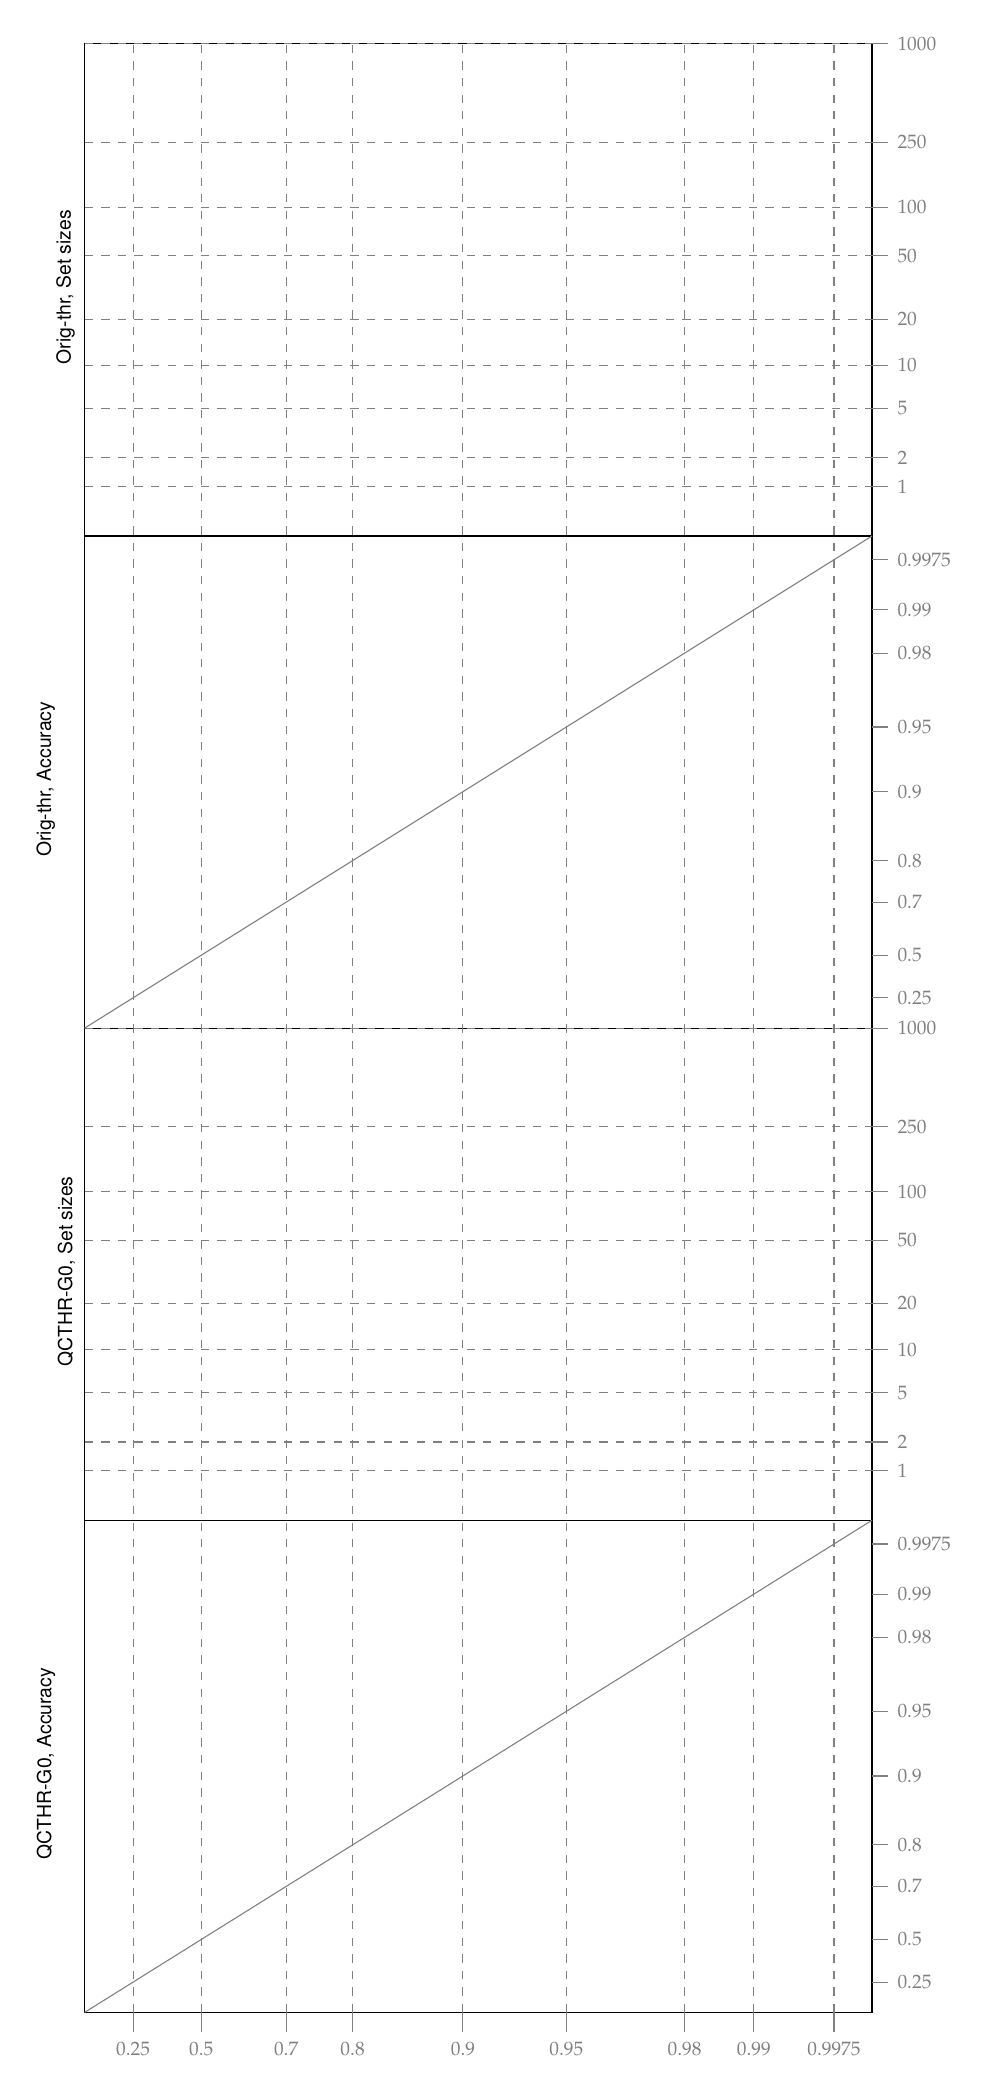
\begin{tikzpicture}[yscale=1.25]\draw (0,0) rectangle (10,20);
\draw (0,5) -- +(10,0);\draw (0,10) -- +(10,0);\node[anchor=east] at (-0.25,2.5) {\rotatebox{90}{\scriptsize \textsf{ QCTHR-G0, Accuracy}}};
\node[anchor=east] at (0,7.5) {\rotatebox{90}{\scriptsize \textsf{ QCTHR-G0, Set sizes}}};
\draw (0,15) -- +(10,0);\node[anchor=east] at (-0.25,12.5) {\rotatebox{90}{\scriptsize \textsf{ Orig-thr, Accuracy}}};
\node[anchor=east] at (0,17.5) {\rotatebox{90}{\scriptsize \textsf{ Orig-thr, Set sizes}}};
\draw[color=black!50!white] (0,0) -- +(10,5);
\draw[color=black!50!white] (0,10) -- +(10,5);
\draw[color=black!50!white] (0.6162074760933258,0) -- +(0,-0.2) node[below] {\scriptsize 0.25};
\draw[color=black!50!white,dashed] (0.6162074760933258,0) -- +(0,20);
\draw[color=black!50!white] (1.4805569683900757,0) -- +(0,-0.2) node[below] {\scriptsize 0.5};
\draw[color=black!50!white,dashed] (1.4805569683900757,0) -- +(0,20);
\draw[color=black!50!white] (2.5592686215798315,0) -- +(0,-0.2) node[below] {\scriptsize 0.7};
\draw[color=black!50!white,dashed] (2.5592686215798315,0) -- +(0,20);
\draw[color=black!50!white] (3.4031572380103423,0) -- +(0,-0.2) node[below] {\scriptsize 0.8};
\draw[color=black!50!white,dashed] (3.4031572380103423,0) -- +(0,20);
\draw[color=black!50!white] (4.804262935175594,0) -- +(0,-0.2) node[below] {\scriptsize 0.9};
\draw[color=black!50!white,dashed] (4.804262935175594,0) -- +(0,20);
\draw[color=black!50!white] (6.117632329015766,0) -- +(0,-0.2) node[below] {\scriptsize 0.95};
\draw[color=black!50!white,dashed] (6.117632329015766,0) -- +(0,20);
\draw[color=black!50!white] (7.619537161252646,0) -- +(0,-0.2) node[below] {\scriptsize 0.98};
\draw[color=black!50!white,dashed] (7.619537161252646,0) -- +(0,20);
\draw[color=black!50!white] (8.49809516776312,0) -- +(0,-0.2) node[below] {\scriptsize 0.99};
\draw[color=black!50!white,dashed] (8.49809516776312,0) -- +(0,20);
\draw[color=black!50!white] (9.516494638655868,0) -- +(0,-0.2) node[below] {\scriptsize 0.9975};
\draw[color=black!50!white,dashed] (9.516494638655868,0) -- +(0,20);
\draw[color=black!50!white] (10,0.3081037380466629) -- +(0.2,0) node[right] {\scriptsize 0.25};
\draw[color=black!50!white] (10,0.7402784841950378) -- +(0.2,0) node[right] {\scriptsize 0.5};
\draw[color=black!50!white] (10,1.2796343107899157) -- +(0.2,0) node[right] {\scriptsize 0.7};
\draw[color=black!50!white] (10,1.7015786190051712) -- +(0.2,0) node[right] {\scriptsize 0.8};
\draw[color=black!50!white] (10,2.402131467587797) -- +(0.2,0) node[right] {\scriptsize 0.9};
\draw[color=black!50!white] (10,3.058816164507883) -- +(0.2,0) node[right] {\scriptsize 0.95};
\draw[color=black!50!white] (10,3.809768580626323) -- +(0.2,0) node[right] {\scriptsize 0.98};
\draw[color=black!50!white] (10,4.24904758388156) -- +(0.2,0) node[right] {\scriptsize 0.99};
\draw[color=black!50!white] (10,4.758247319327934) -- +(0.2,0) node[right] {\scriptsize 0.9975};
\draw[color=black!50!white,dashed] (0,5.501644075308061) -- +(10,0);
\draw[color=black!50!white] (10,5.501644075308061) -- +(0.2,0) node[right] {\scriptsize 1};
\draw[color=black!50!white,dashed] (0,5.795087048072215) -- +(10,0);
\draw[color=black!50!white] (10,5.795087048072215) -- +(0.2,0) node[right] {\scriptsize 2};
\draw[color=black!50!white,dashed] (0,6.296731123380276) -- +(10,0);
\draw[color=black!50!white] (10,6.296731123380276) -- +(0.2,0) node[right] {\scriptsize 5};
\draw[color=black!50!white,dashed] (0,6.735403375422774) -- +(10,0);
\draw[color=black!50!white] (10,6.735403375422774) -- +(0.2,0) node[right] {\scriptsize 10};
\draw[color=black!50!white,dashed] (0,7.203380012009334) -- +(10,0);
\draw[color=black!50!white] (10,7.203380012009334) -- +(0.2,0) node[right] {\scriptsize 20};
\draw[color=black!50!white,dashed] (0,7.845538565427299) -- +(10,0);
\draw[color=black!50!white] (10,7.845538565427299) -- +(0.2,0) node[right] {\scriptsize 50};
\draw[color=black!50!white,dashed] (0,8.340052342470534) -- +(10,0);
\draw[color=black!50!white] (10,8.340052342470534) -- +(0.2,0) node[right] {\scriptsize 100};
\draw[color=black!50!white,dashed] (0,8.998877594899565) -- +(10,0);
\draw[color=black!50!white] (10,8.998877594899565) -- +(0.2,0) node[right] {\scriptsize 250};
\draw[color=black!50!white,dashed] (0,10.0) -- +(10,0);
\draw[color=black!50!white] (10,10.0) -- +(0.2,0) node[right] {\scriptsize 1000};
\draw[color=black!50!white] (10,10.308103738046663) -- +(0.2,0) node[right] {\scriptsize 0.25};
\draw[color=black!50!white] (10,10.740278484195038) -- +(0.2,0) node[right] {\scriptsize 0.5};
\draw[color=black!50!white] (10,11.279634310789916) -- +(0.2,0) node[right] {\scriptsize 0.7};
\draw[color=black!50!white] (10,11.701578619005172) -- +(0.2,0) node[right] {\scriptsize 0.8};
\draw[color=black!50!white] (10,12.402131467587797) -- +(0.2,0) node[right] {\scriptsize 0.9};
\draw[color=black!50!white] (10,13.058816164507883) -- +(0.2,0) node[right] {\scriptsize 0.95};
\draw[color=black!50!white] (10,13.809768580626322) -- +(0.2,0) node[right] {\scriptsize 0.98};
\draw[color=black!50!white] (10,14.24904758388156) -- +(0.2,0) node[right] {\scriptsize 0.99};
\draw[color=black!50!white] (10,14.758247319327934) -- +(0.2,0) node[right] {\scriptsize 0.9975};
\draw[color=black!50!white,dashed] (0,15.50164407530806) -- +(10,0);
\draw[color=black!50!white] (10,15.50164407530806) -- +(0.2,0) node[right] {\scriptsize 1};
\draw[color=black!50!white,dashed] (0,15.795087048072215) -- +(10,0);
\draw[color=black!50!white] (10,15.795087048072215) -- +(0.2,0) node[right] {\scriptsize 2};
\draw[color=black!50!white,dashed] (0,16.296731123380276) -- +(10,0);
\draw[color=black!50!white] (10,16.296731123380276) -- +(0.2,0) node[right] {\scriptsize 5};
\draw[color=black!50!white,dashed] (0,16.735403375422774) -- +(10,0);
\draw[color=black!50!white] (10,16.735403375422774) -- +(0.2,0) node[right] {\scriptsize 10};
\draw[color=black!50!white,dashed] (0,17.203380012009333) -- +(10,0);
\draw[color=black!50!white] (10,17.203380012009333) -- +(0.2,0) node[right] {\scriptsize 20};
\draw[color=black!50!white,dashed] (0,17.845538565427297) -- +(10,0);
\draw[color=black!50!white] (10,17.845538565427297) -- +(0.2,0) node[right] {\scriptsize 50};
\draw[color=black!50!white,dashed] (0,18.340052342470536) -- +(10,0);
\draw[color=black!50!white] (10,18.340052342470536) -- +(0.2,0) node[right] {\scriptsize 100};
\draw[color=black!50!white,dashed] (0,18.998877594899565) -- +(10,0);
\draw[color=black!50!white] (10,18.998877594899565) -- +(0.2,0) node[right] {\scriptsize 250};
\draw[color=black!50!white,dashed] (0,20.0) -- +(10,0);
\draw[color=black!50!white] (10,20.0) -- +(0.2,0) node[right] {\scriptsize 1000};
\end{tikzpicture}\section{Interesting cases found Calibration}
\textbf{Cases filtered:} Interesting cases with large deviation for target probability 0.99


\textbf{Parameter/Probability Combinations considered:}\begin{enumerate}
\item (none)
\end{enumerate}\section{Performance on test data}
\paragraph{Predictor:QCTHR-G2} calibration at alpha=0.01. calibration value={0: 0.9989973774964425, 1: 0.9992372153305972}. Correct: 12223/12500\\
Average set size: 13.7008   Coverage: 0.97784\\
Set size histogram (0..K):\\
0 | 2383 | 1692 | 1146 | 796 | 651 | 555 | 416 | 347 | 303 | 266 | 226 | 222 | 200 | 179 | 157 | 141 | 141 | 128 | 114 | 97 | 84 | 86 | 77 | 97 | 49 | 74 | 62 | 55 | 69 | 43 | 39 | 50 | 41 | 56 | 43 | 59 | 42 | 39 | 36 | 42 | 36 | 41 | 34 | 35 | 33 | 27 | 39 | 24 | 22 | 30 | 34 | 20 | 26 | 26 | 33 | 19 | 14 | 19 | 19 | 18 | 18 | 21 | 22 | 9 | 28 | 16 | 18 | 14 | 28 | 12 | 13 | 13 | 16 | 15 | 15 | 13 | 13 | 12 | 13 | 6 | 5 | 8 | 11 | 14 | 11 | 17 | 9 | 8 | 4 | 9 | 9 | 5 | 5 | 9 | 5 | 5 | 11 | 7 | 8 | 10 | 2 | 5 | 7 | 7 | 6 | 5 | 7 | 1 | 3 | 7 | 6 | 2 | 5 | 6 | 3 | 3 | 5 | 5 | 3 | 4 | 3 | 1 | 1 | 3 | 3 | 2 | 3 | 5 | 3 | 5 | 3 | 2 | 1 | 2 | 2 | 1 | 0 | 2 | 3 | 1 | 0 | 0 | 1 | 1 | 2 | 1 | 1 | 0 | 1 | 0 | 1 | 1 | 2 | 0 | 1 | 0 | 0 | 0 | 0 | 0 | 1 | 1 | 1 | 0 | 1 | 1 | 0 | 1 | 1 | 0 | 0 | 0 | 0 | 1 | 0 | 0 | 0 | 1 | 0 | 0 | 1 | 0 | 0 | 0 | 0 | 0 | 0 | 1 | 0 | 0 | 0 | 0 | 0 | 0 | 1 | 0 | 0 | 0 | 0 | 0 | 1 | 0 | 0 | 0 | 0 | 0 | 0 | 0 | 0 | 0 | 0 | 0 | 0 | 0 | 0 | 0 | 0 | 0 | 0 | 0 | 0 | 0 | 0 | 0 | 0 | 0 | 0 | 0 | 0 | 0 | 0 | 0 | 0 | 0 | 0 | 0 | 0 | 0 | 0 | 0 | 0 | 0 | 0 | 0 | 0 | 0 | 0 | 0 | 0 | 0 | 0 | 0 | 0 | 0 | 0 | 0 | 0 | 0 | 0 | 0 | 0 | 0 | 0 | 0 | 0 | 0 | 0 | 0 | 0 | 0 | 0 | 0 | 0 | 0 | 0 | 0 | 0 | 0 | 0 | 0 | 0 | 0 | 0 | 0 | 0 | 0 | 0 | 0 | 0 | 0 | 0 | 0 | 0 | 0 | 0 | 0 | 0 | 0 | 0 | 0 | 0 | 0 | 0 | 0 | 0 | 0 | 0 | 0 | 0 | 0 | 0 | 0 | 0 | 0 | 0 | 0 | 0 | 0 | 0 | 0 | 0 | 0 | 0 | 0 | 0 | 0 | 0 | 0 | 0 | 0 | 0 | 0 | 0 | 0 | 0 | 0 | 0 | 0 | 0 | 0 | 0 | 0 | 0 | 0 | 0 | 0 | 0 | 0 | 0 | 0 | 0 | 0 | 0 | 0 | 0 | 0 | 0 | 0 | 0 | 0 | 0 | 0 | 0 | 0 | 0 | 0 | 0 | 0 | 0 | 0 | 0 | 0 | 0 | 0 | 0 | 0 | 0 | 0 | 0 | 0 | 0 | 0 | 0 | 0 | 0 | 0 | 0 | 0 | 0 | 0 | 0 | 0 | 0 | 0 | 0 | 0 | 0 | 0 | 0 | 0 | 0 | 0 | 0 | 0 | 0 | 0 | 0 | 0 | 0 | 0 | 0 | 0 | 0 | 0 | 0 | 0 | 0 | 0 | 0 | 0 | 0 | 0 | 0 | 0 | 0 | 0 | 0 | 0 | 0 | 0 | 0 | 0 | 0 | 0 | 0 | 0 | 0 | 0 | 0 | 0 | 0 | 0 | 0 | 0 | 0 | 0 | 0 | 0 | 0 | 0 | 0 | 0 | 0 | 0 | 0 | 0 | 0 | 0 | 0 | 0 | 0 | 0 | 0 | 0 | 0 | 0 | 0 | 0 | 0 | 0 | 0 | 0 | 0 | 0 | 0 | 0 | 0 | 0 | 0 | 0 | 0 | 0 | 0 | 0 | 0 | 0 | 0 | 0 | 0 | 0 | 0 | 0 | 0 | 0 | 0 | 0 | 0 | 0 | 0 | 0 | 0 | 0 | 0 | 0 | 0 | 0 | 0 | 0 | 0 | 0 | 0 | 0 | 0 | 0 | 0 | 0 | 0 | 0 | 0 | 0 | 0 | 0 | 0 | 0 | 0 | 0 | 0 | 0 | 0 | 0 | 0 | 0 | 0 | 0 | 0 | 0 | 0 | 0 | 0 | 0 | 0 | 0 | 0 | 0 | 0 | 0 | 0 | 0 | 0 | 0 | 0 | 0 | 0 | 0 | 0 | 0 | 0 | 0 | 0 | 0 | 0 | 0 | 0 | 0 | 0 | 0 | 0 | 0 | 0 | 0 | 0 | 0 | 0 | 0 | 0 | 0 | 0 | 0 | 0 | 0 | 0 | 0 | 0 | 0 | 0 | 0 | 0 | 0 | 0 | 0 | 0 | 0 | 0 | 0 | 0 | 0 | 0 | 0 | 0 | 0 | 0 | 0 | 0 | 0 | 0 | 0 | 0 | 0 | 0 | 0 | 0 | 0 | 0 | 0 | 0 | 0 | 0 | 0 | 0 | 0 | 0 | 0 | 0 | 0 | 0 | 0 | 0 | 0 | 0 | 0 | 0 | 0 | 0 | 0 | 0 | 0 | 0 | 0 | 0 | 0 | 0 | 0 | 0 | 0 | 0 | 0 | 0 | 0 | 0 | 0 | 0 | 0 | 0 | 0 | 0 | 0 | 0 | 0 | 0 | 0 | 0 | 0 | 0 | 0 | 0 | 0 | 0 | 0 | 0 | 0 | 0 | 0 | 0 | 0 | 0 | 0 | 0 | 0 | 0 | 0 | 0 | 0 | 0 | 0 | 0 | 0 | 0 | 0 | 0 | 0 | 0 | 0 | 0 | 0 | 0 | 0 | 0 | 0 | 0 | 0 | 0 | 0 | 0 | 0 | 0 | 0 | 0 | 0 | 0 | 0 | 0 | 0 | 0 | 0 | 0 | 0 | 0 | 0 | 0 | 0 | 0 | 0 | 0 | 0 | 0 | 0 | 0 | 0 | 0 | 0 | 0 | 0 | 0 | 0 | 0 | 0 | 0 | 0 | 0 | 0 | 0 | 0 | 0 | 0 | 0 | 0 | 0 | 0 | 0 | 0 | 0 | 0 | 0 | 0 | 0 | 0 | 0 | 0 | 0 | 0 | 0 | 0 | 0 | 0 | 0 | 0 | 0 | 0 | 0 | 0 | 0 | 0 | 0 | 0 | 0 | 0 | 0 | 0 | 0 | 0 | 0 | 0 | 0 | 0 | 0 | 0 | 0 | 0 | 0 | 0 | 0 | 0 | 0 | 0 | 0 | 0 | 0 | 0 | 0 | 0 | 0 | 0 | 0 | 0 | 0 | 0 | 0 | 0 | 0 | 0 | 0 | 0 | 0 | 0 | 0 | 0 | 0 | 0 | 0 | 0 | 0 | 0 | 0 | 0 | 0 | 0 | 0 | 0 | 0 | 0 | 0 | 0 | 0 | 0 | 0 | 0 | 0 | 0 | 0 | 0 | 0 | 0 | 0 | 0 | 0 | 0 | 0 | 0 | 0 | 0 | 0 | 0 | 0 | 0 | 0 | 0 | 0 | 0 | 0 | 0 | 0 | 0 | 0 | 0 | 0 | 0 | 0 | 0 | 0 | 0 | 0 | 0 | 0 | 0 | 0 | 0 | 0 | 0 | 0 | 0 | 0 | 0 | 0 | 0 | 0 | 0 | 0 | 0 | 0 | 0 | 0 | 0 | 0 | 0 | 0 | 0 | 0 | 0 | 0 | 0 | 0 | 0 | 0 | 0 | 0 | 0 | 0 | 0 | 0 | 0 | 0 | 0 | 0 | 0 | 0 | 0 | 0 | 0 | 0 | 0 | 0 | 0 | 0 | 0 | 0 | 0 | 0 | 0 | 0 | 0 | 0 | 0 | 0 | 0 | 0 | 0 | 0 | 0 | 0 | 0 | 0 | 0 | 0 | 0 | 0 | 0 | 0 | 0 | 0 | 0 | 0 | 0 | 0 | 0 | 0 | 0 | 0 | 0 | 0 | 0 | 0 | 0 | 0 | 0 | 0 | 0 | 0 | 0 | 0 | 0 | 0 | 0 | 0 | 0 | 0 | 0 | 0 | 0 | 0 | 0 | 0 | 0 | 0 | 0 | 0 | 0 | 0 | 0 | 0 | 0 | 0 | 0 | 0 | 0 | 0 | 0 | 0 | 0 | 0 | 0\\
\paragraph{Metrics for QCTHR-G2}~\\
\begin{tabular}{l r}
\hline
Coverage (target 0.990) & 0.9778 $\pm$ 0.0013 \\
Average set size & 13.701 \\
Median set size & 5.0 \\
Singleton rate (size $=1$) & 0.1906 \\
Large-set rate (size $\geq 250$) & 0.0000 \\
\textbf{SSCV} (worst size-bin gap) & \textbf{0.0308} \\
Class-coverage spread (max$-$min) & 0.3333 \\
Class-coverage std & 0.0475 \\
\textbf{CovGap} (difficulty-conditioned) & \textbf{0.0135} \\
~~Weighted CovGap & 0.0135 \\
~~Worst under-coverage & -0.0388 \\
\hline
\end{tabular}\\[0.5em]
\textsf{\scriptsize Size-stratified coverage (SSCV bins):}\\
\begin{tabular}{l r r}
\hline
Size range & Count & Coverage \\
\hline
1 & 2383 & 0.9924 \\
2--3 & 2838 & 0.9887 \\
4--6 & 2002 & 0.9870 \\
7--10 & 1332 & 0.9700 \\
11--1000 & 3945 & 0.9592 \\
\hline
\end{tabular}\\[0.5em]
\textsf{\scriptsize Difficulty-stratified coverage (CovGap bins, by $1-\max p_{\mathrm{orig}}$):}\\
\begin{tabular}{l r r}
\hline
Difficulty range & Count & Coverage \\
\hline
0.000--0.000 & 1250 & 0.9968 \\
0.000--0.002 & 1250 & 0.9896 \\
0.002--0.008 & 1250 & 0.9856 \\
0.008--0.027 & 1250 & 0.9864 \\
0.027--0.072 & 1250 & 0.9776 \\
0.072--0.164 & 1250 & 0.9792 \\
0.164--0.296 & 1250 & 0.9752 \\
0.296--0.448 & 1250 & 0.9712 \\
0.448--0.614 & 1250 & 0.9656 \\
0.614--0.960 & 1250 & 0.9512 \\
\hline
\end{tabular}\\[0.5em]
\paragraph{Predictor:Orig-thr} calibration at alpha=0.01. calibration value=0.9998482614215284. Correct: 12379/12500\\
Average set size: 34.42904   Coverage: 0.99032\\
Set size histogram (0..K):\\
0 | 1418 | 1181 | 940 | 684 | 571 | 516 | 417 | 352 | 352 | 288 | 238 | 213 | 204 | 196 | 160 | 145 | 146 | 126 | 119 | 127 | 106 | 106 | 90 | 90 | 105 | 83 | 83 | 75 | 52 | 84 | 68 | 63 | 51 | 56 | 48 | 54 | 51 | 46 | 53 | 40 | 38 | 36 | 53 | 28 | 33 | 36 | 43 | 35 | 38 | 25 | 38 | 36 | 27 | 28 | 31 | 28 | 33 | 20 | 24 | 26 | 18 | 24 | 28 | 22 | 19 | 26 | 24 | 24 | 14 | 17 | 27 | 23 | 29 | 23 | 13 | 21 | 23 | 17 | 18 | 13 | 20 | 23 | 19 | 20 | 9 | 12 | 17 | 16 | 22 | 20 | 8 | 19 | 21 | 9 | 18 | 10 | 10 | 13 | 12 | 17 | 12 | 10 | 18 | 14 | 11 | 15 | 16 | 11 | 14 | 18 | 14 | 10 | 9 | 12 | 13 | 12 | 15 | 7 | 11 | 13 | 17 | 18 | 10 | 9 | 7 | 14 | 12 | 8 | 11 | 10 | 5 | 9 | 6 | 8 | 10 | 7 | 10 | 12 | 4 | 9 | 12 | 8 | 6 | 15 | 5 | 3 | 6 | 8 | 12 | 13 | 8 | 7 | 11 | 8 | 9 | 6 | 10 | 9 | 14 | 5 | 6 | 12 | 5 | 10 | 5 | 10 | 14 | 3 | 4 | 8 | 2 | 4 | 8 | 6 | 5 | 6 | 3 | 3 | 8 | 5 | 2 | 3 | 11 | 6 | 6 | 7 | 6 | 6 | 3 | 4 | 3 | 10 | 7 | 9 | 5 | 3 | 7 | 4 | 7 | 5 | 7 | 3 | 10 | 0 | 4 | 1 | 2 | 7 | 3 | 7 | 3 | 1 | 4 | 7 | 8 | 4 | 2 | 0 | 5 | 4 | 5 | 3 | 3 | 1 | 8 | 8 | 6 | 2 | 4 | 7 | 2 | 3 | 3 | 4 | 6 | 3 | 3 | 5 | 4 | 8 | 4 | 3 | 4 | 1 | 1 | 6 | 3 | 3 | 3 | 3 | 5 | 2 | 1 | 2 | 0 | 2 | 4 | 4 | 4 | 1 | 1 | 4 | 2 | 4 | 1 | 2 | 1 | 1 | 1 | 2 | 3 | 2 | 3 | 2 | 2 | 3 | 4 | 1 | 1 | 0 | 4 | 1 | 1 | 2 | 3 | 4 | 4 | 1 | 0 | 2 | 2 | 3 | 1 | 1 | 2 | 2 | 1 | 1 | 1 | 1 | 0 | 0 | 4 | 1 | 3 | 0 | 1 | 2 | 0 | 3 | 1 | 2 | 2 | 3 | 1 | 0 | 2 | 2 | 4 | 1 | 4 | 0 | 2 | 2 | 2 | 3 | 2 | 0 | 1 | 1 | 2 | 1 | 1 | 0 | 0 | 1 | 2 | 1 | 1 | 2 | 3 | 0 | 0 | 0 | 0 | 1 | 0 | 1 | 0 | 0 | 2 | 1 | 0 | 0 | 1 | 0 | 0 | 0 | 1 | 1 | 2 | 0 | 1 | 0 | 1 | 0 | 2 | 1 | 1 | 3 | 0 | 2 | 1 | 0 | 1 | 0 | 0 | 0 | 2 | 0 | 0 | 0 | 1 | 1 | 1 | 0 | 0 | 2 | 1 | 1 | 0 | 2 | 3 | 1 | 3 | 0 | 1 | 0 | 0 | 0 | 2 | 1 | 0 | 1 | 1 | 1 | 1 | 0 | 0 | 0 | 0 | 1 | 2 | 0 | 0 | 0 | 0 | 0 | 0 | 1 | 0 | 0 | 0 | 0 | 0 | 0 | 2 | 0 | 1 | 0 | 0 | 1 | 0 | 0 | 1 | 0 | 1 | 0 | 0 | 0 | 0 | 0 | 0 | 0 | 0 | 1 | 2 | 0 | 0 | 0 | 0 | 1 | 0 | 0 | 0 | 0 | 0 | 0 | 0 | 0 | 0 | 0 | 0 | 0 | 1 | 0 | 0 | 1 | 0 | 0 | 0 | 1 | 1 | 0 | 1 | 0 | 0 | 0 | 0 | 0 | 0 | 0 | 0 | 0 | 0 | 0 | 1 | 0 | 0 | 0 | 0 | 0 | 0 | 0 | 0 | 1 | 1 | 0 | 0 | 0 | 0 | 0 | 0 | 2 | 0 | 0 | 0 | 0 | 0 | 0 | 0 | 0 | 0 | 0 | 0 | 0 | 0 | 0 | 0 | 0 | 0 | 0 | 0 | 1 | 0 | 0 | 0 | 0 | 0 | 0 | 0 | 0 | 0 | 0 | 0 | 0 | 1 | 0 | 0 | 0 | 0 | 0 | 0 | 0 | 0 | 0 | 0 | 0 | 0 | 0 | 0 | 0 | 0 | 0 | 0 | 0 | 0 | 0 | 0 | 0 | 0 | 0 | 0 | 0 | 0 | 0 | 0 | 0 | 0 | 0 | 0 | 0 | 0 | 0 | 0 | 0 | 0 | 0 | 0 | 0 | 0 | 0 | 0 | 0 | 0 | 0 | 0 | 0 | 0 | 0 | 0 | 0 | 0 | 0 | 0 | 0 | 0 | 0 | 0 | 0 | 0 | 0 | 0 | 0 | 0 | 0 | 0 | 1 | 0 | 0 | 0 | 0 | 0 | 0 | 0 | 0 | 0 | 0 | 0 | 0 | 0 | 0 | 0 | 0 | 0 | 0 | 0 | 0 | 0 | 0 | 0 | 0 | 0 | 0 | 0 | 0 | 0 | 0 | 0 | 0 | 0 | 0 | 0 | 0 | 0 | 0 | 0 | 0 | 0 | 0 | 0 | 0 | 0 | 0 | 0 | 0 | 0 | 0 | 0 | 0 | 0 | 0 | 0 | 0 | 0 | 0 | 0 | 0 | 0 | 0 | 0 | 0 | 0 | 0 | 0 | 0 | 0 | 0 | 0 | 0 | 0 | 0 | 0 | 0 | 0 | 0 | 0 | 0 | 0 | 0 | 0 | 0 | 0 | 0 | 0 | 0 | 0 | 0 | 0 | 0 | 0 | 0 | 0 | 0 | 0 | 0 | 0 | 0 | 0 | 0 | 0 | 0 | 0 | 0 | 0 | 0 | 0 | 0 | 0 | 0 | 0 | 0 | 0 | 0 | 0 | 0 | 0 | 0 | 0 | 0 | 0 | 0 | 0 | 0 | 0 | 0 | 0 | 0 | 0 | 0 | 0 | 0 | 0 | 0 | 0 | 0 | 0 | 0 | 0 | 0 | 0 | 0 | 0 | 0 | 0 | 0 | 0 | 0 | 0 | 0 | 0 | 0 | 0 | 0 | 0 | 0 | 0 | 0 | 0 | 0 | 0 | 0 | 0 | 0 | 0 | 0 | 0 | 0 | 0 | 0 | 0 | 0 | 0 | 0 | 0 | 0 | 0 | 0 | 0 | 0 | 0 | 0 | 0 | 0 | 0 | 0 | 0 | 0 | 0 | 0 | 0 | 0 | 0 | 0 | 0 | 0 | 0 | 0 | 0 | 0 | 0 | 0 | 0 | 0 | 0 | 0 | 0 | 0 | 0 | 0 | 0 | 0 | 0 | 0 | 0 | 0 | 0 | 0 | 0 | 0 | 0 | 0 | 0 | 0 | 0 | 0 | 0 | 0 | 0 | 0 | 0 | 0 | 0 | 0 | 0 | 0 | 0 | 0 | 0 | 0 | 0 | 0 | 0 | 0 | 0 | 0 | 0 | 0 | 0 | 0 | 0 | 0 | 0 | 0 | 0 | 0 | 0 | 0 | 0 | 0 | 0 | 0 | 0 | 0 | 0 | 0 | 0 | 0 | 0 | 0 | 0 | 0 | 0 | 0 | 0 | 0 | 0 | 0 | 0 | 0 | 0 | 0 | 0 | 0 | 0 | 0 | 0 | 0 | 0 | 0 | 0 | 0 | 0 | 0 | 0 | 0 | 0 | 0 | 0 | 0 | 0 | 0 | 0 | 0 | 0 | 0 | 0 | 0 | 0 | 0 | 0 | 0 | 0 | 0 | 0 | 0 | 0 | 0 | 0 | 0 | 0 | 0 | 0 | 0 | 0 | 0 | 0 | 0 | 0 | 0 | 0 | 0 | 0 | 0 | 0 | 0 | 0 | 0 | 0 | 0 | 0 | 0 | 0 | 0 | 0 | 0 | 0 | 0 | 0 | 0 | 0 | 0 | 0 | 0 | 0 | 0 | 0 | 0 | 0 | 0 | 0 | 0 | 0 | 0 | 0 | 0 | 0 | 0 | 0 | 0 | 0 | 0 | 0 | 0 | 0 | 0 | 0 | 0 | 0 | 0 | 0 | 0 | 0 | 0 | 0 | 0 | 0 | 0 | 0 | 0\\
\paragraph{Metrics for Orig-thr}~\\
\begin{tabular}{l r}
\hline
Coverage (target 0.990) & 0.9903 $\pm$ 0.0009 \\
Average set size & 34.429 \\
Median set size & 9.0 \\
Singleton rate (size $=1$) & 0.1134 \\
Large-set rate (size $\geq 250$) & 0.0195 \\
\textbf{SSCV} (worst size-bin gap) & \textbf{0.0079} \\
Class-coverage spread (max$-$min) & 0.3333 \\
Class-coverage std & 0.0321 \\
\textbf{CovGap} (difficulty-conditioned) & \textbf{0.0030} \\
~~Weighted CovGap & 0.0030 \\
~~Worst under-coverage & -0.0052 \\
\hline
\end{tabular}\\[0.5em]
\textsf{\scriptsize Size-stratified coverage (SSCV bins):}\\
\begin{tabular}{l r r}
\hline
Size range & Count & Coverage \\
\hline
1 & 1418 & 0.9979 \\
2--3 & 2121 & 0.9925 \\
4--6 & 1771 & 0.9910 \\
7--10 & 1409 & 0.9943 \\
11--1000 & 5781 & 0.9865 \\
\hline
\end{tabular}\\[0.5em]
\textsf{\scriptsize Difficulty-stratified coverage (CovGap bins, by $1-\max p_{\mathrm{orig}}$):}\\
\begin{tabular}{l r r}
\hline
Difficulty range & Count & Coverage \\
\hline
0.000--0.000 & 1250 & 0.9968 \\
0.000--0.002 & 1250 & 0.9944 \\
0.002--0.008 & 1250 & 0.9904 \\
0.008--0.027 & 1250 & 0.9920 \\
0.027--0.072 & 1250 & 0.9888 \\
0.072--0.164 & 1250 & 0.9928 \\
0.164--0.296 & 1250 & 0.9896 \\
0.296--0.448 & 1250 & 0.9872 \\
0.448--0.614 & 1250 & 0.9864 \\
0.614--0.960 & 1250 & 0.9848 \\
\hline
\end{tabular}\\[0.5em]
\subsection{Metric comparison across predictors}
\begin{tabular}{l r r r r r r r r}
\hline
Predictor & Coverage & Avg size & Median & Singleton & Large & SSCV & CovGap & wUnder \\
\hline
QCTHR-G2 & 0.9778 & 13.701 & 5.0 & 0.1906 & 0.0000 & 0.0308 & 0.0135 & -0.0388 \\
Orig-thr & 0.9903 & 34.429 & 9.0 & 0.1134 & 0.0195 & 0.0079 & 0.0030 & -0.0052 \\
\hline
\end{tabular}\\[0.5em]
\textsf{\scriptsize SSCV = worst absolute coverage gap across prediction-set-size strata. CovGap = mean absolute deviation of difficulty-stratified coverage from the target $1-\alpha$. wUnder = worst difficulty-stratum under-coverage; values closer to zero are better.}\\
\section{Interesting cases found Testing}
\textbf{Cases filtered:} Interesting cases with large deviation for target probability 0.99


\textbf{Parameter/Probability Combinations considered:}\begin{enumerate}
\item Calibration Value: None with probability 0.99032
\end{enumerate}
        \end{document}
        